% Created by tikzDevice version 0.12.3.1 on 2021-06-13 12:18:57
% !TEX encoding = UTF-8 Unicode
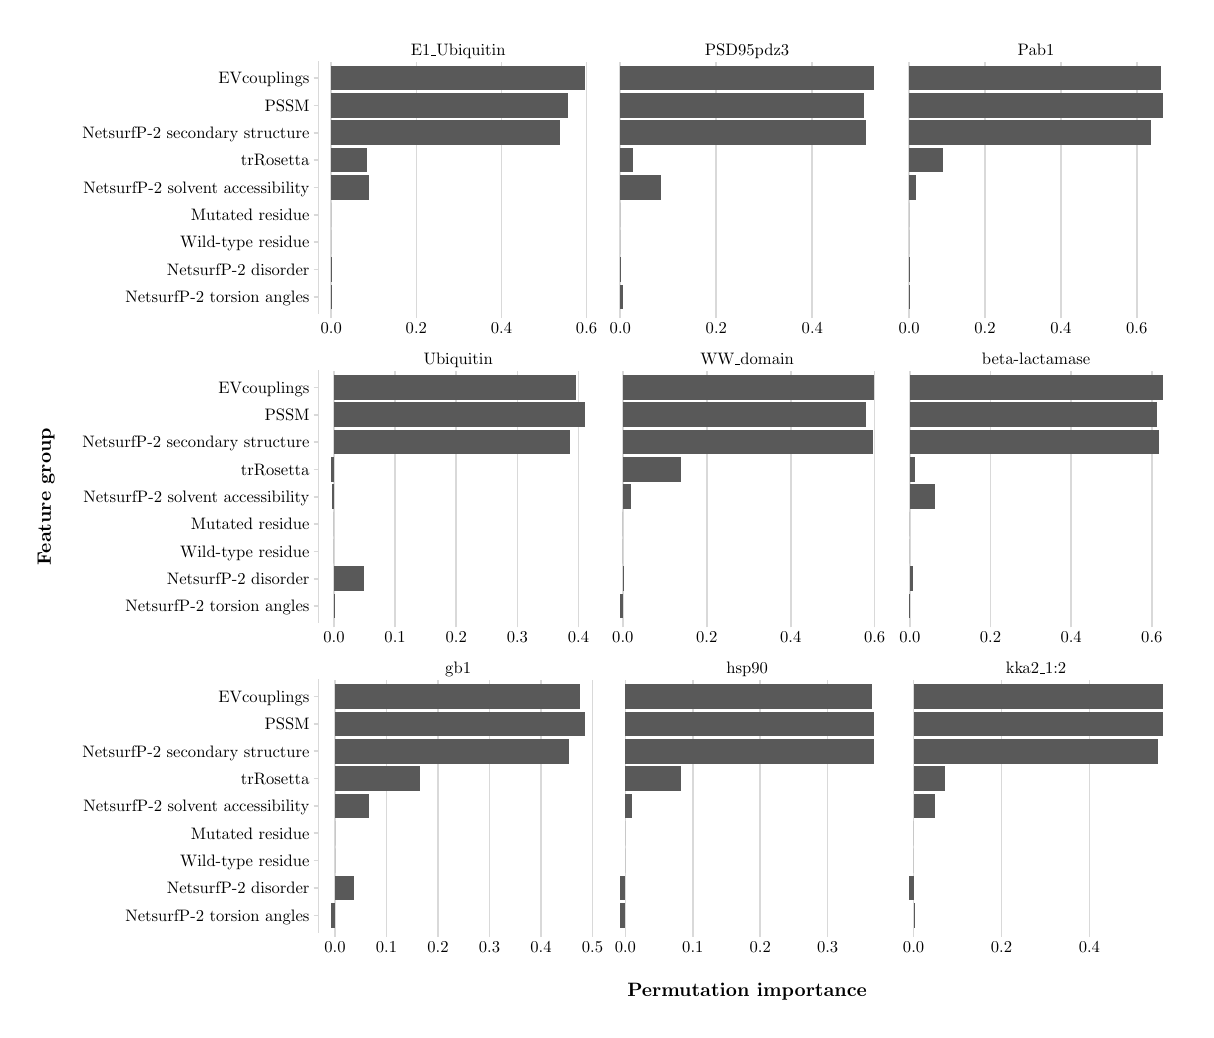
\begin{tikzpicture}[x=1pt,y=1pt]
\definecolor{fillColor}{RGB}{255,255,255}
\path[use as bounding box,fill=fillColor,fill opacity=0.00] (0,0) rectangle (418.34,354.99);
\begin{scope}
\path[clip] (105.09,251.79) rectangle (206.00,342.69);
\definecolor{drawColor}{gray}{0.85}

\path[draw=drawColor,line width= 0.6pt,line join=round] (109.69,251.79) --
	(109.69,342.69);

\path[draw=drawColor,line width= 0.6pt,line join=round] (140.45,251.79) --
	(140.45,342.69);

\path[draw=drawColor,line width= 0.6pt,line join=round] (171.21,251.79) --
	(171.21,342.69);

\path[draw=drawColor,line width= 0.6pt,line join=round] (201.96,251.79) --
	(201.96,342.69);
\definecolor{fillColor}{gray}{0.35}

\path[fill=fillColor] (109.69,302.67) rectangle (122.69,311.57);

\path[fill=fillColor] (109.69,322.43) rectangle (195.31,331.33);

\path[fill=fillColor] (109.69,292.79) rectangle (123.28,301.69);

\path[fill=fillColor] (109.69,312.55) rectangle (192.26,321.45);

\path[fill=fillColor] (109.69,263.15) rectangle (109.70,272.05);

\path[fill=fillColor] (109.68,253.27) rectangle (109.69,262.17);

\path[fill=fillColor] (109.69,332.31) rectangle (201.42,341.21);

\path[fill=fillColor] (109.69,273.03) rectangle (109.69,281.93);

\path[fill=fillColor] (109.69,282.91) rectangle (109.69,291.81);
\end{scope}
\begin{scope}
\path[clip] (105.09,140.05) rectangle (206.00,230.94);
\definecolor{drawColor}{gray}{0.85}

\path[draw=drawColor,line width= 0.6pt,line join=round] (110.68,140.05) --
	(110.68,230.94);

\path[draw=drawColor,line width= 0.6pt,line join=round] (132.77,140.05) --
	(132.77,230.94);

\path[draw=drawColor,line width= 0.6pt,line join=round] (154.86,140.05) --
	(154.86,230.94);

\path[draw=drawColor,line width= 0.6pt,line join=round] (176.95,140.05) --
	(176.95,230.94);

\path[draw=drawColor,line width= 0.6pt,line join=round] (199.04,140.05) --
	(199.04,230.94);
\definecolor{fillColor}{gray}{0.35}

\path[fill=fillColor] (109.68,190.93) rectangle (110.68,199.82);

\path[fill=fillColor] (110.68,210.69) rectangle (201.42,219.58);

\path[fill=fillColor] (110.07,181.05) rectangle (110.68,189.94);

\path[fill=fillColor] (110.68,200.81) rectangle (195.95,209.70);

\path[fill=fillColor] (110.68,151.41) rectangle (121.65,160.30);

\path[fill=fillColor] (110.68,141.53) rectangle (111.20,150.42);

\path[fill=fillColor] (110.68,220.57) rectangle (198.22,229.46);

\path[fill=fillColor] (110.68,161.29) rectangle (110.68,170.18);

\path[fill=fillColor] (110.68,171.17) rectangle (110.68,180.06);
\end{scope}
\begin{scope}
\path[clip] (105.09, 28.30) rectangle (206.00,119.20);
\definecolor{drawColor}{gray}{0.85}

\path[draw=drawColor,line width= 0.6pt,line join=round] (111.07, 28.30) --
	(111.07,119.20);

\path[draw=drawColor,line width= 0.6pt,line join=round] (129.68, 28.30) --
	(129.68,119.20);

\path[draw=drawColor,line width= 0.6pt,line join=round] (148.28, 28.30) --
	(148.28,119.20);

\path[draw=drawColor,line width= 0.6pt,line join=round] (166.88, 28.30) --
	(166.88,119.20);

\path[draw=drawColor,line width= 0.6pt,line join=round] (185.48, 28.30) --
	(185.48,119.20);

\path[draw=drawColor,line width= 0.6pt,line join=round] (204.08, 28.30) --
	(204.08,119.20);
\definecolor{fillColor}{gray}{0.35}

\path[fill=fillColor] (111.07, 79.19) rectangle (141.81, 88.08);

\path[fill=fillColor] (111.07, 98.95) rectangle (201.42,107.84);

\path[fill=fillColor] (111.07, 69.31) rectangle (123.44, 78.20);

\path[fill=fillColor] (111.07, 89.07) rectangle (195.66, 97.96);

\path[fill=fillColor] (111.07, 39.67) rectangle (117.86, 48.56);

\path[fill=fillColor] (109.68, 29.79) rectangle (111.07, 38.68);

\path[fill=fillColor] (111.07,108.82) rectangle (199.51,117.72);

\path[fill=fillColor] (111.07, 49.55) rectangle (111.07, 58.44);

\path[fill=fillColor] (111.07, 59.43) rectangle (111.07, 68.32);
\end{scope}
\begin{scope}
\path[clip] (209.50,251.79) rectangle (310.42,342.69);
\definecolor{drawColor}{gray}{0.85}

\path[draw=drawColor,line width= 0.6pt,line join=round] (214.15,251.79) --
	(214.15,342.69);

\path[draw=drawColor,line width= 0.6pt,line join=round] (248.84,251.79) --
	(248.84,342.69);

\path[draw=drawColor,line width= 0.6pt,line join=round] (283.53,251.79) --
	(283.53,342.69);
\definecolor{fillColor}{gray}{0.35}

\path[fill=fillColor] (214.15,302.67) rectangle (218.58,311.57);

\path[fill=fillColor] (214.15,322.43) rectangle (302.20,331.33);

\path[fill=fillColor] (214.15,292.79) rectangle (228.73,301.69);

\path[fill=fillColor] (214.15,312.55) rectangle (303.00,321.45);

\path[fill=fillColor] (214.09,263.15) rectangle (214.15,272.05);

\path[fill=fillColor] (214.15,253.27) rectangle (215.10,262.17);

\path[fill=fillColor] (214.15,332.31) rectangle (305.83,341.21);

\path[fill=fillColor] (214.15,273.03) rectangle (214.15,281.93);

\path[fill=fillColor] (214.15,282.91) rectangle (214.15,291.81);
\end{scope}
\begin{scope}
\path[clip] (209.50,140.05) rectangle (310.42,230.94);
\definecolor{drawColor}{gray}{0.85}

\path[draw=drawColor,line width= 0.6pt,line join=round] (215.06,140.05) --
	(215.06,230.94);

\path[draw=drawColor,line width= 0.6pt,line join=round] (245.39,140.05) --
	(245.39,230.94);

\path[draw=drawColor,line width= 0.6pt,line join=round] (275.72,140.05) --
	(275.72,230.94);

\path[draw=drawColor,line width= 0.6pt,line join=round] (306.05,140.05) --
	(306.05,230.94);
\definecolor{fillColor}{gray}{0.35}

\path[fill=fillColor] (215.06,190.93) rectangle (236.16,199.82);

\path[fill=fillColor] (215.06,210.69) rectangle (302.93,219.58);

\path[fill=fillColor] (215.06,181.05) rectangle (217.87,189.94);

\path[fill=fillColor] (215.06,200.81) rectangle (305.55,209.70);

\path[fill=fillColor] (215.04,151.41) rectangle (215.06,160.30);

\path[fill=fillColor] (214.09,141.53) rectangle (215.06,150.42);

\path[fill=fillColor] (215.06,220.57) rectangle (305.83,229.46);

\path[fill=fillColor] (215.06,161.29) rectangle (215.06,170.18);

\path[fill=fillColor] (215.06,171.17) rectangle (215.06,180.06);
\end{scope}
\begin{scope}
\path[clip] (209.50, 28.30) rectangle (310.42,119.20);
\definecolor{drawColor}{gray}{0.85}

\path[draw=drawColor,line width= 0.6pt,line join=round] (215.99, 28.30) --
	(215.99,119.20);

\path[draw=drawColor,line width= 0.6pt,line join=round] (240.35, 28.30) --
	(240.35,119.20);

\path[draw=drawColor,line width= 0.6pt,line join=round] (264.70, 28.30) --
	(264.70,119.20);

\path[draw=drawColor,line width= 0.6pt,line join=round] (289.06, 28.30) --
	(289.06,119.20);
\definecolor{fillColor}{gray}{0.35}

\path[fill=fillColor] (215.99, 79.19) rectangle (236.05, 88.08);

\path[fill=fillColor] (215.99, 98.95) rectangle (305.83,107.84);

\path[fill=fillColor] (215.99, 69.31) rectangle (218.42, 78.20);

\path[fill=fillColor] (215.99, 89.07) rectangle (305.64, 97.96);

\path[fill=fillColor] (214.09, 39.67) rectangle (215.99, 48.56);

\path[fill=fillColor] (214.18, 29.79) rectangle (215.99, 38.68);

\path[fill=fillColor] (215.99,108.82) rectangle (305.07,117.72);

\path[fill=fillColor] (215.99, 49.55) rectangle (215.99, 58.44);

\path[fill=fillColor] (215.99, 59.43) rectangle (215.99, 68.32);
\end{scope}
\begin{scope}
\path[clip] (313.92,251.79) rectangle (414.84,342.69);
\definecolor{drawColor}{gray}{0.85}

\path[draw=drawColor,line width= 0.6pt,line join=round] (318.52,251.79) --
	(318.52,342.69);

\path[draw=drawColor,line width= 0.6pt,line join=round] (345.93,251.79) --
	(345.93,342.69);

\path[draw=drawColor,line width= 0.6pt,line join=round] (373.35,251.79) --
	(373.35,342.69);

\path[draw=drawColor,line width= 0.6pt,line join=round] (400.76,251.79) --
	(400.76,342.69);
\definecolor{fillColor}{gray}{0.35}

\path[fill=fillColor] (318.52,302.67) rectangle (330.70,311.57);

\path[fill=fillColor] (318.52,322.43) rectangle (410.25,331.33);

\path[fill=fillColor] (318.52,292.79) rectangle (320.99,301.69);

\path[fill=fillColor] (318.52,312.55) rectangle (406.00,321.45);

\path[fill=fillColor] (318.51,263.15) rectangle (318.52,272.05);

\path[fill=fillColor] (318.52,253.27) rectangle (318.61,262.17);

\path[fill=fillColor] (318.52,332.31) rectangle (409.46,341.21);

\path[fill=fillColor] (318.52,273.03) rectangle (318.52,281.93);

\path[fill=fillColor] (318.52,282.91) rectangle (318.52,291.81);
\end{scope}
\begin{scope}
\path[clip] (313.92,140.05) rectangle (414.84,230.94);
\definecolor{drawColor}{gray}{0.85}

\path[draw=drawColor,line width= 0.6pt,line join=round] (318.79,140.05) --
	(318.79,230.94);

\path[draw=drawColor,line width= 0.6pt,line join=round] (347.93,140.05) --
	(347.93,230.94);

\path[draw=drawColor,line width= 0.6pt,line join=round] (377.07,140.05) --
	(377.07,230.94);

\path[draw=drawColor,line width= 0.6pt,line join=round] (406.21,140.05) --
	(406.21,230.94);
\definecolor{fillColor}{gray}{0.35}

\path[fill=fillColor] (318.79,190.93) rectangle (320.81,199.82);

\path[fill=fillColor] (318.79,210.69) rectangle (408.01,219.58);

\path[fill=fillColor] (318.79,181.05) rectangle (327.94,189.94);

\path[fill=fillColor] (318.79,200.81) rectangle (408.77,209.70);

\path[fill=fillColor] (318.79,151.41) rectangle (319.84,160.30);

\path[fill=fillColor] (318.51,141.53) rectangle (318.79,150.42);

\path[fill=fillColor] (318.79,220.57) rectangle (410.25,229.46);

\path[fill=fillColor] (318.79,161.29) rectangle (318.79,170.18);

\path[fill=fillColor] (318.79,171.17) rectangle (318.79,180.06);
\end{scope}
\begin{scope}
\path[clip] (313.92, 28.30) rectangle (414.84,119.20);
\definecolor{drawColor}{gray}{0.85}

\path[draw=drawColor,line width= 0.6pt,line join=round] (320.13, 28.30) --
	(320.13,119.20);

\path[draw=drawColor,line width= 0.6pt,line join=round] (351.89, 28.30) --
	(351.89,119.20);

\path[draw=drawColor,line width= 0.6pt,line join=round] (383.65, 28.30) --
	(383.65,119.20);
\definecolor{fillColor}{gray}{0.35}

\path[fill=fillColor] (320.13, 79.19) rectangle (331.43, 88.08);

\path[fill=fillColor] (320.13, 98.95) rectangle (410.09,107.84);

\path[fill=fillColor] (320.13, 69.31) rectangle (327.87, 78.20);

\path[fill=fillColor] (320.13, 89.07) rectangle (408.33, 97.96);

\path[fill=fillColor] (318.51, 39.67) rectangle (320.13, 48.56);

\path[fill=fillColor] (320.13, 29.79) rectangle (320.27, 38.68);

\path[fill=fillColor] (320.13,108.82) rectangle (410.25,117.72);

\path[fill=fillColor] (320.13, 49.55) rectangle (320.13, 58.44);

\path[fill=fillColor] (320.13, 59.43) rectangle (320.13, 68.32);
\end{scope}
\begin{scope}
\path[clip] (105.09,119.20) rectangle (206.00,128.00);
\definecolor{drawColor}{RGB}{0,0,0}

\node[text=drawColor,anchor=base,inner sep=0pt, outer sep=0pt, scale=  0.60] at (155.55,121.53) {gb1};
\end{scope}
\begin{scope}
\path[clip] (209.50,119.20) rectangle (310.42,128.00);
\definecolor{drawColor}{RGB}{0,0,0}

\node[text=drawColor,anchor=base,inner sep=0pt, outer sep=0pt, scale=  0.60] at (259.96,121.53) {hsp90};
\end{scope}
\begin{scope}
\path[clip] (313.92,119.20) rectangle (414.84,128.00);
\definecolor{drawColor}{RGB}{0,0,0}

\node[text=drawColor,anchor=base,inner sep=0pt, outer sep=0pt, scale=  0.60] at (364.38,121.53) {kka2\_1:2};
\end{scope}
\begin{scope}
\path[clip] (105.09,230.94) rectangle (206.00,239.74);
\definecolor{drawColor}{RGB}{0,0,0}

\node[text=drawColor,anchor=base,inner sep=0pt, outer sep=0pt, scale=  0.60] at (155.55,233.28) {Ubiquitin};
\end{scope}
\begin{scope}
\path[clip] (209.50,230.94) rectangle (310.42,239.74);
\definecolor{drawColor}{RGB}{0,0,0}

\node[text=drawColor,anchor=base,inner sep=0pt, outer sep=0pt, scale=  0.60] at (259.96,233.28) {WW\_domain};
\end{scope}
\begin{scope}
\path[clip] (313.92,230.94) rectangle (414.84,239.74);
\definecolor{drawColor}{RGB}{0,0,0}

\node[text=drawColor,anchor=base,inner sep=0pt, outer sep=0pt, scale=  0.60] at (364.38,233.28) {beta-lactamase};
\end{scope}
\begin{scope}
\path[clip] (105.09,342.69) rectangle (206.00,351.49);
\definecolor{drawColor}{RGB}{0,0,0}

\node[text=drawColor,anchor=base,inner sep=0pt, outer sep=0pt, scale=  0.60] at (155.55,345.02) {E1\_Ubiquitin};
\end{scope}
\begin{scope}
\path[clip] (209.50,342.69) rectangle (310.42,351.49);
\definecolor{drawColor}{RGB}{0,0,0}

\node[text=drawColor,anchor=base,inner sep=0pt, outer sep=0pt, scale=  0.60] at (259.96,345.02) {PSD95pdz3};
\end{scope}
\begin{scope}
\path[clip] (313.92,342.69) rectangle (414.84,351.49);
\definecolor{drawColor}{RGB}{0,0,0}

\node[text=drawColor,anchor=base,inner sep=0pt, outer sep=0pt, scale=  0.60] at (364.38,345.02) {Pab1};
\end{scope}
\begin{scope}
\path[clip] (  0.00,  0.00) rectangle (418.34,354.99);
\definecolor{drawColor}{gray}{0.85}

\path[draw=drawColor,line width= 0.6pt,line join=round] (111.07, 26.55) --
	(111.07, 28.30);

\path[draw=drawColor,line width= 0.6pt,line join=round] (129.68, 26.55) --
	(129.68, 28.30);

\path[draw=drawColor,line width= 0.6pt,line join=round] (148.28, 26.55) --
	(148.28, 28.30);

\path[draw=drawColor,line width= 0.6pt,line join=round] (166.88, 26.55) --
	(166.88, 28.30);

\path[draw=drawColor,line width= 0.6pt,line join=round] (185.48, 26.55) --
	(185.48, 28.30);

\path[draw=drawColor,line width= 0.6pt,line join=round] (204.08, 26.55) --
	(204.08, 28.30);
\end{scope}
\begin{scope}
\path[clip] (  0.00,  0.00) rectangle (418.34,354.99);
\definecolor{drawColor}{RGB}{0,0,0}

\node[text=drawColor,anchor=base,inner sep=0pt, outer sep=0pt, scale=  0.60] at (111.07, 20.92) {0.0};

\node[text=drawColor,anchor=base,inner sep=0pt, outer sep=0pt, scale=  0.60] at (129.68, 20.92) {0.1};

\node[text=drawColor,anchor=base,inner sep=0pt, outer sep=0pt, scale=  0.60] at (148.28, 20.92) {0.2};

\node[text=drawColor,anchor=base,inner sep=0pt, outer sep=0pt, scale=  0.60] at (166.88, 20.92) {0.3};

\node[text=drawColor,anchor=base,inner sep=0pt, outer sep=0pt, scale=  0.60] at (185.48, 20.92) {0.4};

\node[text=drawColor,anchor=base,inner sep=0pt, outer sep=0pt, scale=  0.60] at (204.08, 20.92) {0.5};
\end{scope}
\begin{scope}
\path[clip] (  0.00,  0.00) rectangle (418.34,354.99);
\definecolor{drawColor}{gray}{0.85}

\path[draw=drawColor,line width= 0.6pt,line join=round] (215.99, 26.55) --
	(215.99, 28.30);

\path[draw=drawColor,line width= 0.6pt,line join=round] (240.35, 26.55) --
	(240.35, 28.30);

\path[draw=drawColor,line width= 0.6pt,line join=round] (264.70, 26.55) --
	(264.70, 28.30);

\path[draw=drawColor,line width= 0.6pt,line join=round] (289.06, 26.55) --
	(289.06, 28.30);
\end{scope}
\begin{scope}
\path[clip] (  0.00,  0.00) rectangle (418.34,354.99);
\definecolor{drawColor}{RGB}{0,0,0}

\node[text=drawColor,anchor=base,inner sep=0pt, outer sep=0pt, scale=  0.60] at (215.99, 20.92) {0.0};

\node[text=drawColor,anchor=base,inner sep=0pt, outer sep=0pt, scale=  0.60] at (240.35, 20.92) {0.1};

\node[text=drawColor,anchor=base,inner sep=0pt, outer sep=0pt, scale=  0.60] at (264.70, 20.92) {0.2};

\node[text=drawColor,anchor=base,inner sep=0pt, outer sep=0pt, scale=  0.60] at (289.06, 20.92) {0.3};
\end{scope}
\begin{scope}
\path[clip] (  0.00,  0.00) rectangle (418.34,354.99);
\definecolor{drawColor}{gray}{0.85}

\path[draw=drawColor,line width= 0.6pt,line join=round] (320.13, 26.55) --
	(320.13, 28.30);

\path[draw=drawColor,line width= 0.6pt,line join=round] (351.89, 26.55) --
	(351.89, 28.30);

\path[draw=drawColor,line width= 0.6pt,line join=round] (383.65, 26.55) --
	(383.65, 28.30);
\end{scope}
\begin{scope}
\path[clip] (  0.00,  0.00) rectangle (418.34,354.99);
\definecolor{drawColor}{RGB}{0,0,0}

\node[text=drawColor,anchor=base,inner sep=0pt, outer sep=0pt, scale=  0.60] at (320.13, 20.92) {0.0};

\node[text=drawColor,anchor=base,inner sep=0pt, outer sep=0pt, scale=  0.60] at (351.89, 20.92) {0.2};

\node[text=drawColor,anchor=base,inner sep=0pt, outer sep=0pt, scale=  0.60] at (383.65, 20.92) {0.4};
\end{scope}
\begin{scope}
\path[clip] (  0.00,  0.00) rectangle (418.34,354.99);
\definecolor{drawColor}{gray}{0.85}

\path[draw=drawColor,line width= 0.6pt,line join=round] (110.68,138.30) --
	(110.68,140.05);

\path[draw=drawColor,line width= 0.6pt,line join=round] (132.77,138.30) --
	(132.77,140.05);

\path[draw=drawColor,line width= 0.6pt,line join=round] (154.86,138.30) --
	(154.86,140.05);

\path[draw=drawColor,line width= 0.6pt,line join=round] (176.95,138.30) --
	(176.95,140.05);

\path[draw=drawColor,line width= 0.6pt,line join=round] (199.04,138.30) --
	(199.04,140.05);
\end{scope}
\begin{scope}
\path[clip] (  0.00,  0.00) rectangle (418.34,354.99);
\definecolor{drawColor}{RGB}{0,0,0}

\node[text=drawColor,anchor=base,inner sep=0pt, outer sep=0pt, scale=  0.60] at (110.68,132.67) {0.0};

\node[text=drawColor,anchor=base,inner sep=0pt, outer sep=0pt, scale=  0.60] at (132.77,132.67) {0.1};

\node[text=drawColor,anchor=base,inner sep=0pt, outer sep=0pt, scale=  0.60] at (154.86,132.67) {0.2};

\node[text=drawColor,anchor=base,inner sep=0pt, outer sep=0pt, scale=  0.60] at (176.95,132.67) {0.3};

\node[text=drawColor,anchor=base,inner sep=0pt, outer sep=0pt, scale=  0.60] at (199.04,132.67) {0.4};
\end{scope}
\begin{scope}
\path[clip] (  0.00,  0.00) rectangle (418.34,354.99);
\definecolor{drawColor}{gray}{0.85}

\path[draw=drawColor,line width= 0.6pt,line join=round] (215.06,138.30) --
	(215.06,140.05);

\path[draw=drawColor,line width= 0.6pt,line join=round] (245.39,138.30) --
	(245.39,140.05);

\path[draw=drawColor,line width= 0.6pt,line join=round] (275.72,138.30) --
	(275.72,140.05);

\path[draw=drawColor,line width= 0.6pt,line join=round] (306.05,138.30) --
	(306.05,140.05);
\end{scope}
\begin{scope}
\path[clip] (  0.00,  0.00) rectangle (418.34,354.99);
\definecolor{drawColor}{RGB}{0,0,0}

\node[text=drawColor,anchor=base,inner sep=0pt, outer sep=0pt, scale=  0.60] at (215.06,132.67) {0.0};

\node[text=drawColor,anchor=base,inner sep=0pt, outer sep=0pt, scale=  0.60] at (245.39,132.67) {0.2};

\node[text=drawColor,anchor=base,inner sep=0pt, outer sep=0pt, scale=  0.60] at (275.72,132.67) {0.4};

\node[text=drawColor,anchor=base,inner sep=0pt, outer sep=0pt, scale=  0.60] at (306.05,132.67) {0.6};
\end{scope}
\begin{scope}
\path[clip] (  0.00,  0.00) rectangle (418.34,354.99);
\definecolor{drawColor}{gray}{0.85}

\path[draw=drawColor,line width= 0.6pt,line join=round] (318.79,138.30) --
	(318.79,140.05);

\path[draw=drawColor,line width= 0.6pt,line join=round] (347.93,138.30) --
	(347.93,140.05);

\path[draw=drawColor,line width= 0.6pt,line join=round] (377.07,138.30) --
	(377.07,140.05);

\path[draw=drawColor,line width= 0.6pt,line join=round] (406.21,138.30) --
	(406.21,140.05);
\end{scope}
\begin{scope}
\path[clip] (  0.00,  0.00) rectangle (418.34,354.99);
\definecolor{drawColor}{RGB}{0,0,0}

\node[text=drawColor,anchor=base,inner sep=0pt, outer sep=0pt, scale=  0.60] at (318.79,132.67) {0.0};

\node[text=drawColor,anchor=base,inner sep=0pt, outer sep=0pt, scale=  0.60] at (347.93,132.67) {0.2};

\node[text=drawColor,anchor=base,inner sep=0pt, outer sep=0pt, scale=  0.60] at (377.07,132.67) {0.4};

\node[text=drawColor,anchor=base,inner sep=0pt, outer sep=0pt, scale=  0.60] at (406.21,132.67) {0.6};
\end{scope}
\begin{scope}
\path[clip] (  0.00,  0.00) rectangle (418.34,354.99);
\definecolor{drawColor}{gray}{0.85}

\path[draw=drawColor,line width= 0.6pt,line join=round] (109.69,250.04) --
	(109.69,251.79);

\path[draw=drawColor,line width= 0.6pt,line join=round] (140.45,250.04) --
	(140.45,251.79);

\path[draw=drawColor,line width= 0.6pt,line join=round] (171.21,250.04) --
	(171.21,251.79);

\path[draw=drawColor,line width= 0.6pt,line join=round] (201.96,250.04) --
	(201.96,251.79);
\end{scope}
\begin{scope}
\path[clip] (  0.00,  0.00) rectangle (418.34,354.99);
\definecolor{drawColor}{RGB}{0,0,0}

\node[text=drawColor,anchor=base,inner sep=0pt, outer sep=0pt, scale=  0.60] at (109.69,244.41) {0.0};

\node[text=drawColor,anchor=base,inner sep=0pt, outer sep=0pt, scale=  0.60] at (140.45,244.41) {0.2};

\node[text=drawColor,anchor=base,inner sep=0pt, outer sep=0pt, scale=  0.60] at (171.21,244.41) {0.4};

\node[text=drawColor,anchor=base,inner sep=0pt, outer sep=0pt, scale=  0.60] at (201.96,244.41) {0.6};
\end{scope}
\begin{scope}
\path[clip] (  0.00,  0.00) rectangle (418.34,354.99);
\definecolor{drawColor}{gray}{0.85}

\path[draw=drawColor,line width= 0.6pt,line join=round] (214.15,250.04) --
	(214.15,251.79);

\path[draw=drawColor,line width= 0.6pt,line join=round] (248.84,250.04) --
	(248.84,251.79);

\path[draw=drawColor,line width= 0.6pt,line join=round] (283.53,250.04) --
	(283.53,251.79);
\end{scope}
\begin{scope}
\path[clip] (  0.00,  0.00) rectangle (418.34,354.99);
\definecolor{drawColor}{RGB}{0,0,0}

\node[text=drawColor,anchor=base,inner sep=0pt, outer sep=0pt, scale=  0.60] at (214.15,244.41) {0.0};

\node[text=drawColor,anchor=base,inner sep=0pt, outer sep=0pt, scale=  0.60] at (248.84,244.41) {0.2};

\node[text=drawColor,anchor=base,inner sep=0pt, outer sep=0pt, scale=  0.60] at (283.53,244.41) {0.4};
\end{scope}
\begin{scope}
\path[clip] (  0.00,  0.00) rectangle (418.34,354.99);
\definecolor{drawColor}{gray}{0.85}

\path[draw=drawColor,line width= 0.6pt,line join=round] (318.52,250.04) --
	(318.52,251.79);

\path[draw=drawColor,line width= 0.6pt,line join=round] (345.93,250.04) --
	(345.93,251.79);

\path[draw=drawColor,line width= 0.6pt,line join=round] (373.35,250.04) --
	(373.35,251.79);

\path[draw=drawColor,line width= 0.6pt,line join=round] (400.76,250.04) --
	(400.76,251.79);
\end{scope}
\begin{scope}
\path[clip] (  0.00,  0.00) rectangle (418.34,354.99);
\definecolor{drawColor}{RGB}{0,0,0}

\node[text=drawColor,anchor=base,inner sep=0pt, outer sep=0pt, scale=  0.60] at (318.52,244.41) {0.0};

\node[text=drawColor,anchor=base,inner sep=0pt, outer sep=0pt, scale=  0.60] at (345.93,244.41) {0.2};

\node[text=drawColor,anchor=base,inner sep=0pt, outer sep=0pt, scale=  0.60] at (373.35,244.41) {0.4};

\node[text=drawColor,anchor=base,inner sep=0pt, outer sep=0pt, scale=  0.60] at (400.76,244.41) {0.6};
\end{scope}
\begin{scope}
\path[clip] (  0.00,  0.00) rectangle (418.34,354.99);
\definecolor{drawColor}{gray}{0.85}

\path[draw=drawColor,line width= 0.6pt,line join=round,line cap=rect] (105.09,251.79) --
	(105.09,342.69);
\end{scope}
\begin{scope}
\path[clip] (  0.00,  0.00) rectangle (418.34,354.99);
\definecolor{drawColor}{RGB}{0,0,0}

\node[text=drawColor,anchor=base east,inner sep=0pt, outer sep=0pt, scale=  0.60] at (101.84,255.65) {NetsurfP-2 torsion angles};

\node[text=drawColor,anchor=base east,inner sep=0pt, outer sep=0pt, scale=  0.60] at (101.84,265.53) {NetsurfP-2 disorder};

\node[text=drawColor,anchor=base east,inner sep=0pt, outer sep=0pt, scale=  0.60] at (101.84,275.41) {Wild-type residue};

\node[text=drawColor,anchor=base east,inner sep=0pt, outer sep=0pt, scale=  0.60] at (101.84,285.29) {Mutated residue};

\node[text=drawColor,anchor=base east,inner sep=0pt, outer sep=0pt, scale=  0.60] at (101.84,295.17) {NetsurfP-2 solvent accessibility};

\node[text=drawColor,anchor=base east,inner sep=0pt, outer sep=0pt, scale=  0.60] at (101.84,305.05) {trRosetta};

\node[text=drawColor,anchor=base east,inner sep=0pt, outer sep=0pt, scale=  0.60] at (101.84,314.93) {NetsurfP-2 secondary structure};

\node[text=drawColor,anchor=base east,inner sep=0pt, outer sep=0pt, scale=  0.60] at (101.84,324.81) {PSSM};

\node[text=drawColor,anchor=base east,inner sep=0pt, outer sep=0pt, scale=  0.60] at (101.84,334.69) {EVcouplings};
\end{scope}
\begin{scope}
\path[clip] (  0.00,  0.00) rectangle (418.34,354.99);
\definecolor{drawColor}{gray}{0.85}

\path[draw=drawColor,line width= 0.6pt,line join=round] (103.34,257.72) --
	(105.09,257.72);

\path[draw=drawColor,line width= 0.6pt,line join=round] (103.34,267.60) --
	(105.09,267.60);

\path[draw=drawColor,line width= 0.6pt,line join=round] (103.34,277.48) --
	(105.09,277.48);

\path[draw=drawColor,line width= 0.6pt,line join=round] (103.34,287.36) --
	(105.09,287.36);

\path[draw=drawColor,line width= 0.6pt,line join=round] (103.34,297.24) --
	(105.09,297.24);

\path[draw=drawColor,line width= 0.6pt,line join=round] (103.34,307.12) --
	(105.09,307.12);

\path[draw=drawColor,line width= 0.6pt,line join=round] (103.34,317.00) --
	(105.09,317.00);

\path[draw=drawColor,line width= 0.6pt,line join=round] (103.34,326.88) --
	(105.09,326.88);

\path[draw=drawColor,line width= 0.6pt,line join=round] (103.34,336.76) --
	(105.09,336.76);
\end{scope}
\begin{scope}
\path[clip] (  0.00,  0.00) rectangle (418.34,354.99);
\definecolor{drawColor}{gray}{0.85}

\path[draw=drawColor,line width= 0.6pt,line join=round,line cap=rect] (105.09,140.05) --
	(105.09,230.94);
\end{scope}
\begin{scope}
\path[clip] (  0.00,  0.00) rectangle (418.34,354.99);
\definecolor{drawColor}{RGB}{0,0,0}

\node[text=drawColor,anchor=base east,inner sep=0pt, outer sep=0pt, scale=  0.60] at (101.84,143.91) {NetsurfP-2 torsion angles};

\node[text=drawColor,anchor=base east,inner sep=0pt, outer sep=0pt, scale=  0.60] at (101.84,153.79) {NetsurfP-2 disorder};

\node[text=drawColor,anchor=base east,inner sep=0pt, outer sep=0pt, scale=  0.60] at (101.84,163.67) {Wild-type residue};

\node[text=drawColor,anchor=base east,inner sep=0pt, outer sep=0pt, scale=  0.60] at (101.84,173.55) {Mutated residue};

\node[text=drawColor,anchor=base east,inner sep=0pt, outer sep=0pt, scale=  0.60] at (101.84,183.43) {NetsurfP-2 solvent accessibility};

\node[text=drawColor,anchor=base east,inner sep=0pt, outer sep=0pt, scale=  0.60] at (101.84,193.31) {trRosetta};

\node[text=drawColor,anchor=base east,inner sep=0pt, outer sep=0pt, scale=  0.60] at (101.84,203.19) {NetsurfP-2 secondary structure};

\node[text=drawColor,anchor=base east,inner sep=0pt, outer sep=0pt, scale=  0.60] at (101.84,213.07) {PSSM};

\node[text=drawColor,anchor=base east,inner sep=0pt, outer sep=0pt, scale=  0.60] at (101.84,222.95) {EVcouplings};
\end{scope}
\begin{scope}
\path[clip] (  0.00,  0.00) rectangle (418.34,354.99);
\definecolor{drawColor}{gray}{0.85}

\path[draw=drawColor,line width= 0.6pt,line join=round] (103.34,145.98) --
	(105.09,145.98);

\path[draw=drawColor,line width= 0.6pt,line join=round] (103.34,155.86) --
	(105.09,155.86);

\path[draw=drawColor,line width= 0.6pt,line join=round] (103.34,165.74) --
	(105.09,165.74);

\path[draw=drawColor,line width= 0.6pt,line join=round] (103.34,175.62) --
	(105.09,175.62);

\path[draw=drawColor,line width= 0.6pt,line join=round] (103.34,185.50) --
	(105.09,185.50);

\path[draw=drawColor,line width= 0.6pt,line join=round] (103.34,195.38) --
	(105.09,195.38);

\path[draw=drawColor,line width= 0.6pt,line join=round] (103.34,205.26) --
	(105.09,205.26);

\path[draw=drawColor,line width= 0.6pt,line join=round] (103.34,215.14) --
	(105.09,215.14);

\path[draw=drawColor,line width= 0.6pt,line join=round] (103.34,225.02) --
	(105.09,225.02);
\end{scope}
\begin{scope}
\path[clip] (  0.00,  0.00) rectangle (418.34,354.99);
\definecolor{drawColor}{gray}{0.85}

\path[draw=drawColor,line width= 0.6pt,line join=round,line cap=rect] (105.09, 28.30) --
	(105.09,119.20);
\end{scope}
\begin{scope}
\path[clip] (  0.00,  0.00) rectangle (418.34,354.99);
\definecolor{drawColor}{RGB}{0,0,0}

\node[text=drawColor,anchor=base east,inner sep=0pt, outer sep=0pt, scale=  0.60] at (101.84, 32.17) {NetsurfP-2 torsion angles};

\node[text=drawColor,anchor=base east,inner sep=0pt, outer sep=0pt, scale=  0.60] at (101.84, 42.05) {NetsurfP-2 disorder};

\node[text=drawColor,anchor=base east,inner sep=0pt, outer sep=0pt, scale=  0.60] at (101.84, 51.93) {Wild-type residue};

\node[text=drawColor,anchor=base east,inner sep=0pt, outer sep=0pt, scale=  0.60] at (101.84, 61.81) {Mutated residue};

\node[text=drawColor,anchor=base east,inner sep=0pt, outer sep=0pt, scale=  0.60] at (101.84, 71.68) {NetsurfP-2 solvent accessibility};

\node[text=drawColor,anchor=base east,inner sep=0pt, outer sep=0pt, scale=  0.60] at (101.84, 81.56) {trRosetta};

\node[text=drawColor,anchor=base east,inner sep=0pt, outer sep=0pt, scale=  0.60] at (101.84, 91.44) {NetsurfP-2 secondary structure};

\node[text=drawColor,anchor=base east,inner sep=0pt, outer sep=0pt, scale=  0.60] at (101.84,101.32) {PSSM};

\node[text=drawColor,anchor=base east,inner sep=0pt, outer sep=0pt, scale=  0.60] at (101.84,111.20) {EVcouplings};
\end{scope}
\begin{scope}
\path[clip] (  0.00,  0.00) rectangle (418.34,354.99);
\definecolor{drawColor}{gray}{0.85}

\path[draw=drawColor,line width= 0.6pt,line join=round] (103.34, 34.23) --
	(105.09, 34.23);

\path[draw=drawColor,line width= 0.6pt,line join=round] (103.34, 44.11) --
	(105.09, 44.11);

\path[draw=drawColor,line width= 0.6pt,line join=round] (103.34, 53.99) --
	(105.09, 53.99);

\path[draw=drawColor,line width= 0.6pt,line join=round] (103.34, 63.87) --
	(105.09, 63.87);

\path[draw=drawColor,line width= 0.6pt,line join=round] (103.34, 73.75) --
	(105.09, 73.75);

\path[draw=drawColor,line width= 0.6pt,line join=round] (103.34, 83.63) --
	(105.09, 83.63);

\path[draw=drawColor,line width= 0.6pt,line join=round] (103.34, 93.51) --
	(105.09, 93.51);

\path[draw=drawColor,line width= 0.6pt,line join=round] (103.34,103.39) --
	(105.09,103.39);

\path[draw=drawColor,line width= 0.6pt,line join=round] (103.34,113.27) --
	(105.09,113.27);
\end{scope}
\begin{scope}
\path[clip] (  0.00,  0.00) rectangle (418.34,354.99);
\definecolor{drawColor}{RGB}{0,0,0}

\node[text=drawColor,anchor=base,inner sep=0pt, outer sep=0pt, scale=  0.70] at (259.96,  4.86) {\bfseries Permutation importance};
\end{scope}
\begin{scope}
\path[clip] (  0.00,  0.00) rectangle (418.34,354.99);
\definecolor{drawColor}{RGB}{0,0,0}

\node[text=drawColor,rotate= 90.00,anchor=base,inner sep=0pt, outer sep=0pt, scale=  0.70] at (  8.39,185.50) {\bfseries Feature group};
\end{scope}
\end{tikzpicture}%
